\documentclass[10pt,letterpaper]{article}
\usepackage[margin=0.78in,headheight=14pt]{geometry}
\usepackage[T1]{fontenc}
\usepackage{lmodern,amsmath,amssymb,booktabs,array,tabularx,microtype}
\usepackage{tikz}
\usetikzlibrary{arrows.meta,positioning,calc}
\usepackage{xcolor,enumitem,fancyhdr,hyperref}
\definecolor{ink}{HTML}{18354A}
\definecolor{accent}{HTML}{176B79}
\hypersetup{colorlinks=true,linkcolor=accent,citecolor=accent,urlcolor=accent,pdftitle={SpatialReadout: multiscale delta-rule memory and a final spatial ConvGRU},pdfauthor={Visual Attention and Working Memory project}}
\pagestyle{fancy}\fancyhf{}\fancyhead[L]{\small SpatialReadout: architecture and decision logic}\fancyhead[R]{\small Source-audited technical paper}\fancyfoot[C]{\thepage}
\setlength{\parindent}{0pt}\setlength{\parskip}{5pt}
\renewcommand{\tabularxcolumn}[1]{>{\raggedright\arraybackslash}p{#1}}
\setlist{nosep,leftmargin=*}
\newcommand{\R}{\mathbb{R}}
\newcommand{\cat}{\mathbin\Vert}
\newcommand{\src}[1]{\textcolor{accent}{\textsf{[#1]}}}
\newcommand{\takeaway}[1]{\par\smallskip\noindent\textbf{Takeaway.} #1}
\newcommand{\psection}[1]{\clearpage\section{#1}}
\begin{document}
\thispagestyle{empty}
{\color{ink}\LARGE\bfseries SpatialReadout: Multiscale Delta-Rule Memory\\[3pt] and a Final Spatial ConvGRU\par}
\vspace{8pt}
{\large A step-by-step guide to the computation and its limits}\par
\vspace{4pt}
{\small Visual Attention and Working Memory project\quad\textbullet\quad Local source snapshot, 29 September 2026}
\vspace{8pt}
\begin{abstract}
\noindent This paper specifies the current \texttt{SpatialReadout} model, rather than its historical global-GRU predecessor or an isolated KDA module. Centered, three-frame RGB stacks pass through four convolutional blocks. Three spatial Kimi Delta Attention (KDA) accumulators, interleaved at $25\times25$, $13\times13$, and $7\times7$, contribute local associative memory to the feedforward hierarchy. The deepest $160\times7\times7$ field is projected to 64 channels and integrated by a final convolutional gated recurrent unit (ConvGRU). Only its terminal $64\times7\times7$ state is flattened and projected to 256 features for a task-specific linear head. An independent CPU constructor audit gives \textbf{1,383,028 trainable parameters}. We derive the exact decay--correction--read update, its signed temporal coefficients, and the implemented write/reset convention. The principal design decision is to postpone \emph{global} compression until after final recurrence, while retaining spatially organized encoder memory. This supplies an inductive bias, not proof of better retention, comparison learning, or biological equivalence. We distinguish documented design intent from plausible but untested explanations, and separate the current fresh-origin training lineage from an earlier warm-start branch. No training, trained-model inference, or new behavioral experiment was performed for this paper.
\end{abstract}
\section{Scope and scientific question}
\textbf{Reader question: what does this model make possible, and what has actually been shown?}
Visual working-memory tasks require an observer to encode evidence, retain task-relevant information, and convert that information into a report. These requirements are not interchangeable: a representation may contain a cue without applying its meaning, or retain sensory information without learning the required comparison. An architecture description should therefore explain what computations are available without treating their availability as evidence that training discovered them.

The present observer combines two kinds of recurrence. The encoder carries matrix-valued associative states at three spatial scales; a final ConvGRU carries a feature field at the coarsest scale. The motivating question is whether a spatially structured final recurrent substrate is a more suitable place to integrate the encoder's output than a small vector produced by flattening and projecting \emph{before} recurrence. The implementation makes this substitution without adding a controller, top-down feedback, a hand-designed comparator, a transformer, or spatial softmax attention.\src{S1,S2}

The source authority is the current model and its imported definitions, not the older September KDA report. Historical \texttt{README.md}, \texttt{BRIEF.md}, and journal entries record the original warm-start experiment; the current \texttt{FreshRun} worker constructs every learned tensor anew, and \texttt{ContinuationRun} restores that same fresh-origin model at update 7,739. Retained Python member names support historical migration but do not imply old learned-weight inheritance in the fresh run.\src{S1,S4,S5,S8}

This is an architecture paper, not a report of the paused neuroscience study. Source inspection, algebra, parameter counting, and PDF checks are the evidence presented here. No validation score is treated as current live status, and the authorized continuation target is not represented as completed training.

\takeaway{This paper explains the available computation, not a demonstrated cognitive ability. Read the diagram as a dataflow map, then follow a single memory update before interpreting its history.}

\psection{A reading key: indices, shapes, and kinds of quantity}
\textbf{Reader question: which symbols are learned, and which are computed anew?}
A model has learned weights that persist across episodes and activation states that are recomputed during each episode. A memory matrix here belongs to the second category. Its entries are not additional trainable weights. Finally, we will derive diagnostic matrices from the actual updates; these are algebraic bookkeeping, not extra network layers.

\textbf{Indices.} An episode has $\mathcal T$ frames, with time $t=0,\ldots,\mathcal T-1$ and initial recurrent state at $t=-1$. $B$ is the number of episodes in a batch. We omit the batch index when explaining one episode. The three memory-bearing scales have $s=1,2,3$, corresponding to CNN blocks 2, 3, 4, respectively. At scale $s$, $p$ is a spatial grid site and $j\in\{1,2\}$ is a KDA head. A head is one parallel association mechanism, not an output task head. The task identifier is $a$; its classifier has $K_a$ output classes. Later, $\tau$ will denote an earlier source time, not a different episode.

\begin{tabularx}{\linewidth}{@{}lX@{}}\toprule
Quantity & Shape and status (one episode)\\\midrule
$X_t,\bar X_t,x_t$ & Raw RGB frame, centered frame: $3\times100\times100$; stacked input: $9\times100\times100$. Input-derived.\\
$H_t^s$ & CNN field: $C_s\times L_s\times L_s$, with $(C_s,L_s)=(64,25),(96,13),(128,7)$. Computed activation.\\
$U_t^s,O_t^s$ & Projected input and emitted memory field: $32\times L_s\times L_s$. Computed activations.\\
$S_t^{s,p,j}$ & $8\times16$ recurrent matrix. Rows are key coordinates, columns value coordinates. Starts at zero.\\
$q_t,k_t,v_t$ & Column query/key vectors in $\R^8$, value in $\R^{16}$, generated from current features at one scale/site/head.\\
$\alpha_t,\beta_t$ & Generated gates: an eight-vector of row retentions and one scalar write fraction, respectively.\\
$z_t,h_t,w_t,r_t$ & Final projected field, hidden state, write/reset gates: each $64\times7\times7$.\\
$W_{\cdot},b_{\cdot}$ & Learned weights and biases; dimensions are specified at their operations. Shared across time and (for convolutions) sites.\\\bottomrule
\end{tabularx}

\textbf{Operations.} Superscript $\mathsf T$ means transpose, not a time index. For column vectors $u,v$ of the same length, $u^{\mathsf T}v=\sum_i u_i v_i$ is a dot product: one number. In contrast, $uv^{\mathsf T}$ is an outer product: a matrix whose entry $(i,m)$ is $u_i v_m$. Ordinary juxtaposition denotes matrix multiplication. $\odot$ is elementwise multiplication of equal-shaped fields (or explicitly broadcast gates); $\cat$ joins channel lists. $*$ denotes a spatial convolution, not any of these three products. $I_d$ is the $d\times d$ identity matrix; $\operatorname{diag}(u)$ puts vector entries on a diagonal and zeros elsewhere.

ReLU replaces negative entries by zero; $\sigma(x)=1/(1+e^{-x})$ maps each real entry to $(0,1)$; $\tanh$ maps each to $(-1,1)$. A vector's $\lVert\cdot\rVert_2$ is its Euclidean length. Flattening, written $\operatorname{vec}$, lists all entries in a fixed order without first averaging them.
\takeaway{Weights define the rule; inputs generate queries, values, and gates; recurrent states carry the episode. The transport matrix introduced later is derived from these quantities, never separately learned.}

\psection{End-to-end computation: follow one frame}
\textbf{Reader question: where can earlier images affect the final report?}
The main path carries the present image upward. Three side branches carry local associative states across time; a final spatial recurrent field integrates their deepest output. Only the terminal state is classified.

\begin{figure}[h!]
\centering
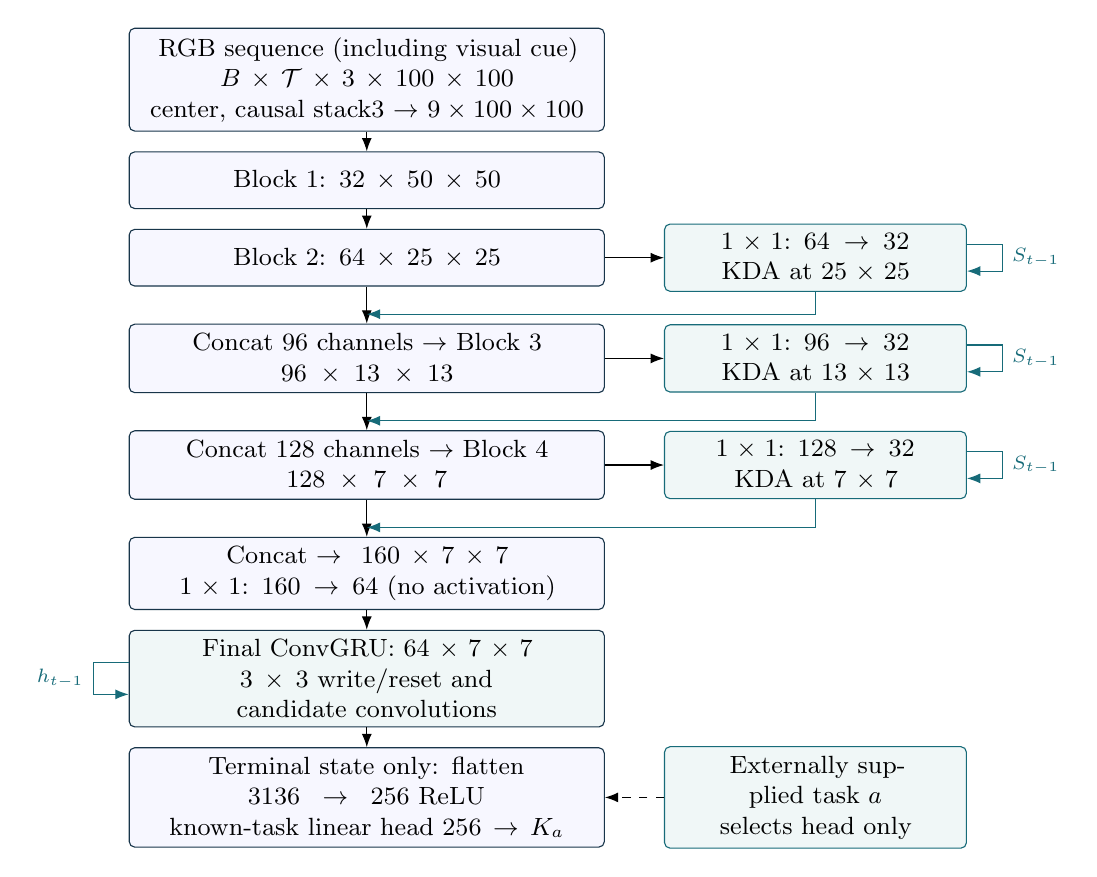
\begin{tikzpicture}[font=\small,>=Latex,box/.style={draw=ink,rounded corners=2pt,fill=blue!3,align=center,minimum height=0.72cm,text width=5.8cm},mem/.style={draw=accent,rounded corners=2pt,fill=teal!6,align=center,text width=3.6cm,minimum height=0.78cm},node distance=0.25cm]
\node[box] (input) {RGB sequence (including visual cue)\\$B\times\mathcal T\times3\times100\times100$\\center, causal stack3 $\rightarrow9\times100\times100$};
\node[box,below=of input] (b1) {Block 1: $32\times50\times50$};
\node[box,below=of b1] (b2) {Block 2: $64\times25\times25$};
\node[mem,right=0.75cm of b2] (m1) {$1\times1$: $64\to32$\\KDA at $25\times25$};
\node[box,below=0.47cm of b2] (b3) {Concat $96$ channels $\to$ Block 3\\$96\times13\times13$};
\node[mem,right=0.75cm of b3] (m2) {$1\times1$: $96\to32$\\KDA at $13\times13$};
\node[box,below=0.47cm of b3] (b4) {Concat $128$ channels $\to$ Block 4\\$128\times7\times7$};
\node[mem,right=0.75cm of b4] (m3) {$1\times1$: $128\to32$\\KDA at $7\times7$};
\node[box,below=0.47cm of b4] (proj) {Concat $\to160\times7\times7$\\$1\times1$: $160\to64$ (no activation)};
\node[box,below=of proj,fill=teal!6] (gru) {Final ConvGRU: $64\times7\times7$\\$3\times3$ write/reset and candidate convolutions};
\node[box,below=of gru] (head) {Terminal state only: \mbox{flatten} $3136\to256$ ReLU\\known-task linear head $256\to K_a$};
\node[mem,right=0.75cm of head] (task) {Externally supplied task $a$\\selects head only};
\draw[->,dashed] (task.west)--(head.east);
\foreach \a/\b in {input/b1,b1/b2,b2/b3,b3/b4,b4/proj,proj/gru,gru/head}{\draw[->] (\a)--(\b);}
\foreach \a/\b/\c in {b2/m1/b3,b3/m2/b4,b4/m3/proj}{\draw[->] (\a.east)--(\b.west);\draw[->,accent] (\b.south)|- ($(\c.north)+(0,0.12)$);\draw[->,accent] ($(\b.east)+(0,0.17)$) -- ++(0.45,0) -- node[right,font=\scriptsize] {$S_{t-1}$} ++(0,-0.34) -- ($(\b.east)+(0,-0.17)$);}
\draw[->,accent] ($(gru.west)+(0,0.20)$) -- ++(-0.45,0) -- node[left,font=\scriptsize] {$h_{t-1}$} ++(0,-0.40) -- ($(gru.west)+(0,-0.20)$);
\end{tikzpicture}
\caption{One causal time step, repeated for every presented frame. Side branches emit 32 channels and retain separate matrix states; they are not global attention layers. Loops indicate state carried from the preceding update. The last readout is applied only after the final step. Batch dimensions are omitted within the diagram.}
\end{figure}

The cue is part of the rendered image. Its location or meaning must affect the shared trunk through learned image processing. The externally supplied task name takes a separate route: it selects the output vocabulary, without telling the trunk the target or answer. There is no learned task-ID inference module.\src{S1,S7}
\takeaway{There are four recurrent pathways, not a single global attention map. The final task-known classifier is distinct from interpreting an endogenous visual cue.}

\psection{Sensory interface and the multiscale encoder}
\textbf{Reader question: what does one update actually see, and how is its spatial grid reduced?}
\subsection{Causal frame stacking has a specific boundary condition}
The suite supplies float32 images in $[0,1]$, laid out as $B\times\mathcal T\times3\times100\times100$. Centering subtracts $0.5$; it does not divide by $0.5$. For zero-based $t$, define
\begin{equation}
\bar X_t=\begin{cases}X_t-0.5,&t\geq0,\\0,&t<0,\end{cases}
\qquad x_t=\bar X_{t-2}\cat\bar X_{t-1}\cat\bar X_t .
\end{equation}
Here $\cat$ concatenates channels in oldest-to-current order. Padding is created \emph{after} centering, so missing history is zero in centered coordinates (equivalent to raw midgray), not centered black. The first input is $[0,0,X_0-0.5]$ and the second is $[0,X_0-0.5,X_1-0.5]$. No future image enters an earlier update.\src{S2,S6}

Stacking supplies adjacent-frame evidence, potentially useful for changes and motion; that rationale is not a measured benefit here. The first two nominal blank updates can still expose earlier stimulus images. A retention test must distinguish recurrent memory from access through this explicit window.

\subsection{Four blocks, three interleaved memories}
Each block is a biased convolution followed by GroupNorm with eight groups and ReLU. The verified GroupNorm epsilon is $10^{-5}$ and the normalization has learned per-channel scale and shift. The first convolution has kernel 5, stride 2, padding 2; all remaining block convolutions use kernel 3, stride 2, padding 1. There is no pooling.\src{S2}\par
\begin{table}[h!]
\centering\small
\begin{tabular}{@{}lllr@{}}\toprule
Stage & Input channels & Output field & Parameters\\\midrule
Block 1: Conv5/GN/ReLU & 9 & $32\times50\times50$ & 7,296\\
Block 2: Conv3/GN/ReLU & 32 & $64\times25\times25$ & 18,624\\
Projection 1; KDA 1 & $64\to32$ & $32\times25\times25$ & $2,080+24,754$\\
Block 3: Conv3/GN/ReLU & $64+32=96$ & $96\times13\times13$ & 83,232\\
Projection 2; KDA 2 & $96\to32$ & $32\times13\times13$ & $3,104+24,754$\\
Block 4: Conv3/GN/ReLU & $96+32=128$ & $128\times7\times7$ & 147,840\\
Projection 3; KDA 3 & $128\to32$ & $32\times7\times7$ & $4,128+24,754$\\\bottomrule
\end{tabular}
\caption{Constructor-verified counts; output sizes are analytically propagated from the actual convolution attributes. Each projection is a biased $1\times1$ convolution. No trained forward pass was needed.}
\end{table}
At a site $p$, the biased pointwise projection is explicitly
\begin{equation}
U_t^s(p)=W_{\mathrm{proj},s}H_t^s(p)+b_{\mathrm{proj},s},\quad
W_{\mathrm{proj},s}\in\R^{32\times C_s},\ b_{\mathrm{proj},s}\in\R^{32}.
\end{equation}
It mixes channels at that site, not neighboring sites: 64 numbers become 32 at scale 1 while the $25\times25$ grid remains. $U_t^s$ drives the KDA update; the next block receives $H_t^s\cat O_t^s$. Thus the next scale sees current features alongside memory emissions; the deepest concatenation is $160\times7\times7$. The three modules have distinct weights and states.

A convolution instead combines channels \emph{and} a local spatial neighborhood with the same kernel at each site. For side length $n$, kernel width $\kappa$, padding $\pi$, and stride $d$ (all block dilations are one), the output side is $\lfloor(n+2\pi-\kappa)/d\rfloor+1$. Thus block 3 takes side 25 to $\lfloor(25+2-3)/2\rfloor+1=13$, not a new set of 13 objects.

GroupNorm avoids batch-dependent normalization statistics, consistent with the small physical microbatch used in training \cite{gn}. It does, however, aggregate within channel groups \emph{over spatial positions}. Therefore ``local KDA state'' does not mean the entire encoder is strictly spatially isolated: convolutional neighborhoods, GroupNorm statistics, and subsequent layers couple information across the field.
\takeaway{Spatial organization survives the encoder, but resolution and channels are already compressed. ``Compression after recurrence'' means postponing the large global flatten/projection, not eliminating every bottleneck.}

\psection{One KDA update: prepare, decay, correct, read}
\textbf{Reader question: how can a matrix act as an associative memory?}
Fix one scale $s$, site $p$, and head $j$, and suppress these indices. Think of $S\in\R^{8\times16}$ as a table that maps a key direction to a predicted value via $S^{\mathsf T}k$. This is an analogy to an addressable notebook, not a claim that a key is an object identity or a value is an angle. The channels are learned features; their semantic content is not established by the architecture.

\subsection{First generate the instructions for this update}
The projected 32-channel field enters a biased $3\times3$ convolution with padding 1: 82 output channels, reshaped to $B\times L_s\times L_s\times2\times41$. Each head's 41 numbers split into raw query $\tilde q_t\in\R^8$, raw key $\tilde k_t\in\R^8$, value $v_t\in\R^{16}$, raw retention $\tilde\alpha_t\in\R^8$, and raw write strength $\tilde\beta_t\in\R$. Tildes here mark the values before normalization or a sigmoid.\src{S3}
\begin{equation}
q_t=\frac{\tilde q_t}{\max(\lVert\tilde q_t\rVert_2,10^{-6})},\quad
k_t=\frac{\tilde k_t}{\max(\lVert\tilde k_t\rVert_2,10^{-6})},\quad
\alpha_t=\sigma(\tilde\alpha_t),\quad\beta_t=\sigma(\tilde\beta_t).
\end{equation}
The key specifies the direction whose stored prediction is corrected; the value supplies the desired new feature vector in that direction. The query specifies the direction read \emph{after} correction, and need not equal the key. Normalized queries/keys have length one except near zero, where the safeguard permits a shorter vector. Values are neither normalized nor restricted to be positive.

\subsection{Then execute four operations in a fixed order}
All states start at $S_{-1}=0$. Define $D_t=\operatorname{diag}(\alpha_t)\in\R^{8\times8}$. The decayed state $\bar S_t$, prediction $\widehat v_t$, error $e_t$, and read $o_t$ are computed as follows:
\begin{align}
\bar S_t &=D_tS_{t-1}, &&\bar S_t\in\R^{8\times16}, \label{eq:decay}\\
\widehat v_t&=\bar S_t^{\mathsf T}k_t,\qquad e_t=v_t-\widehat v_t,
&&\widehat v_t,e_t\in\R^{16},\\
S_t&=\bar S_t+\beta_t k_te_t^{\mathsf T}, &&S_t\in\R^{8\times16},\label{eq:write}\\
o_t&=S_t^{\mathsf T}q_t, &&o_t\in\R^{16}.\label{eq:read}
\end{align}
\textbf{Decay:} row $i$ is multiplied by $\alpha_{t,i}$, leaving its 16 columns scaled together. \textbf{Predict:} the key weights those rows and sums them to predict 16 values. \textbf{Correct:} the outer product distributes the error across rows in proportion to the key, with strength $\beta_t$. \textbf{Read:} the query weights the \emph{updated} rows. There is no spatial softmax or summation over other sites in these four lines.

For explicit indices, with key row $i=1,\ldots,8$ and value column $m=1,\ldots,16$,
\begin{equation}
\widehat v_{t,m}=\sum_{i=1}^{8}\alpha_{t,i}S_{t-1,i m}k_{t,i},\quad
S_{t,i m}=\alpha_{t,i}S_{t-1,i m}+\beta_t k_{t,i}e_{t,m}.
\end{equation}
The two heads' reads concatenate into 32 channels. A biased $1\times1$ output convolution mixes them to form $O_t^s$; there is no extra output normalization or nonlinearity. Its weight is $32\times32$ at each site, with a 32-vector bias. The packed convolution has 23,698 parameters and the output convolution 1,056, totaling 24,754 per module.
\takeaway{KDA writes a prediction error, not the whole incoming value unconditionally. The next page computes every operation with small numbers.}

\psection{A worked two-by-two memory, with no hidden steps}
\textbf{Reader question: what do decay and corrective writing actually change?}
This is a hand-selected arithmetic example with two key and two value coordinates, not the model's actual $8\times16$ head and not a trained-model result. All keys and queries below have unit length; gates lie strictly between zero and one. Start with $S_{-1}=0$. At time 0 choose
\begin{equation}
k_0=q_0=\begin{bmatrix}1\\0\end{bmatrix},\quad
v_0=\begin{bmatrix}2\\4\end{bmatrix},\quad
\alpha_0=\begin{bmatrix}1/2\\3/4\end{bmatrix},\quad\beta_0=1/2.
\end{equation}
Decay leaves zero, so $\widehat v_0=0$ and $e_0=v_0$. The first correction and read are
\begin{equation}
S_0=\tfrac12\begin{bmatrix}1\\0\end{bmatrix}\begin{bmatrix}2&4\end{bmatrix}
=\begin{bmatrix}1&2\\0&0\end{bmatrix},\qquad o_0=\begin{bmatrix}1\\2\end{bmatrix}.
\end{equation}
Only the first row changes because the second key coordinate is zero. The write fraction is one half, so the first prediction moves halfway from zero to the desired value.

At time 1 choose a different key and a query that reads the second row:
\begin{equation}
k_1=\begin{bmatrix}3/5\\4/5\end{bmatrix},\quad q_1=\begin{bmatrix}0\\1\end{bmatrix},\quad
v_1=\begin{bmatrix}2\\0\end{bmatrix},\quad
\alpha_1=\begin{bmatrix}1/2\\3/4\end{bmatrix},\quad\beta_1=1/2.
\end{equation}
\textbf{1. Decay.} Scale row 1 by one half and row 2 by three quarters:
\begin{equation}
\bar S_1=\begin{bmatrix}1/2&0\\0&3/4\end{bmatrix}
\begin{bmatrix}1&2\\0&0\end{bmatrix}=\begin{bmatrix}1/2&1\\0&0\end{bmatrix}.
\end{equation}
\textbf{2. Predict and subtract.} The key weights the two rows:
\begin{equation}
\widehat v_1=\begin{bmatrix}1/2&0\\1&0\end{bmatrix}\begin{bmatrix}3/5\\4/5\end{bmatrix}
=\begin{bmatrix}3/10\\3/5\end{bmatrix},\qquad
e_1=\begin{bmatrix}2\\0\end{bmatrix}-\begin{bmatrix}3/10\\3/5\end{bmatrix}
=\begin{bmatrix}17/10\\-3/5\end{bmatrix}.
\end{equation}
\textbf{3. Write only the correction.} The second error coordinate is negative because the old memory predicted a positive value where the new desired value is zero:
\begin{equation}
\beta_1 k_1e_1^{\mathsf T}=\tfrac12\begin{bmatrix}3/5\\4/5\end{bmatrix}
\begin{bmatrix}17/10&-3/5\end{bmatrix}
=\begin{bmatrix}51/100&-9/50\\17/25&-6/25\end{bmatrix}.
\end{equation}
\textbf{4. Add and read.} Add that correction to the decayed matrix, then select the query direction:
\begin{equation}
S_1=\begin{bmatrix}101/100&41/50\\17/25&-6/25\end{bmatrix},\qquad
o_1=S_1^{\mathsf T}\begin{bmatrix}0\\1\end{bmatrix}
=\begin{bmatrix}17/25\\-6/25\end{bmatrix}.
\end{equation}
\takeaway{Positive gates do not force positive stored features or reads. Exact rational Python arithmetic in \texttt{verify\_toy.py} checks these values and a third update, without constructing or executing a model.}

\psection{Deriving the transition, rather than naming it}
\textbf{Reader question: where does the matrix multiplying the old state come from?}
The four-step implementation above is the starting point. We now rewrite the \emph{same} update to separate what happens to the old matrix from the incoming value. This is algebra, not an additional learned layer.

Substitute the prediction error into the write, and transpose the product carefully:
\begin{align}
S_t&=D_tS_{t-1}+\beta_t k_t\bigl(v_t-(D_tS_{t-1})^{\mathsf T}k_t\bigr)^{\mathsf T}\\
&=D_tS_{t-1}+\beta_t k_t\bigl(v_t^{\mathsf T}-k_t^{\mathsf T}D_tS_{t-1}\bigr)\\
&=D_tS_{t-1}-\beta_t k_tk_t^{\mathsf T}D_tS_{t-1}+\beta_t k_tv_t^{\mathsf T}\\
&=\underbrace{(I_8-\beta_t k_tk_t^{\mathsf T})D_t}_{\text{acts on the old state}}S_{t-1}
+\underbrace{\beta_t k_tv_t^{\mathsf T}}_{\text{incoming-value term}}.
\end{align}
Only \emph{now} define the shorter names $A_t\in\R^{8\times8}$ and $J_t\in\R^{8\times16}$:
\begin{equation}
A_t=(I_8-\beta_t k_tk_t^{\mathsf T})D_t,\qquad J_t=\beta_t k_tv_t^{\mathsf T},\qquad
S_t=A_tS_{t-1}+J_t.\label{eq:transition}
\end{equation}
Neither $A_t$ nor $J_t$ is a free parameter. Both are determined by this update's generated quantities. $J_t$ alone is not the implemented corrective write: part of the correction to old predictions is now inside $A_t$.

\subsection{Why the multiplication order matters}
A matrix product acts from right to left: $D_t$ decays first; $(I_8-\beta_t k_tk_t^{\mathsf T})$ then removes part of the old prediction along the current key. Reversing them changes the computation when different rows have different retentions. The toy's second update gives
\begin{equation}
A_1=\begin{bmatrix}41/100&-9/50\\-3/25&51/100\end{bmatrix},\qquad
J_1=\begin{bmatrix}3/5&0\\4/5&0\end{bmatrix}.
\end{equation}
The two off-diagonal entries differ precisely because the two columns inherit different diagonal decay factors. The Python receipt checks $A_1S_0+J_1=S_1$ against the direct error-correction calculation.

\subsection{Why this is error correction}
Multiply the original write by $k_t$ after transposing. Since $k_t^{\mathsf T}k_t=\lVert k_t\rVert_2^2$,
\begin{align}
S_t^{\mathsf T}k_t
&=\widehat v_t+\beta_t e_t(k_t^{\mathsf T}k_t)\\
&=(1-\beta_t)\widehat v_t+\beta_t v_t\quad\text{if }\lVert k_t\rVert_2=1.
\end{align}
Thus the prediction at a unit key moves a fraction $\beta_t$ toward the current value, rather than growing by the full value every time. For a shorter key, that fraction is $\beta_t\lVert k_t\rVert_2^2$.

This diagonal-gated delta-rule form matches Kimi Linear Eq.~1 \cite{kda}; it does not import that paper's language model, hybrid full attention, mixture of experts, or accelerator kernel. Here it is an explicit small spatial recurrence.\src{S3}
\takeaway{$A_t$ is the derived one-update transformation of old memory. It is not the CNN projection, which has its own learned weight $W_{\mathrm{proj},s}$ and bias.}

\psection{From three updates to a temporal read decomposition}
\textbf{Reader question: how can an earlier value still contribute now?}
Start at zero and substitute the preceding state, one update at a time:
\begin{align}
S_{-1}&=0,\\
S_0&=A_0\,0+J_0=J_0,\\
S_1&=A_1S_0+J_1=A_1J_0+J_1,\\
S_2&=A_2S_1+J_2=A_2(A_1J_0+J_1)+J_2\\
&=A_2A_1J_0+A_2J_1+J_2.
\end{align}
The value introduced at time 0 passes through transitions 1 and 2; the value introduced at time 1 passes only through transition 2. The current write has no later transition to pass through. This pattern, not an independently assumed matrix, motivates a name for the intervening product.

\textbf{Definition after the expansion.} For source time $\tau\leq t$, define the \emph{retention transport} $\mathsf T_{t\leftarrow\tau}\in\R^{8\times8}$:
\begin{equation}
\mathsf T_{t\leftarrow\tau}=A_tA_{t-1}\cdots A_{\tau+1}\quad(\tau<t),\qquad
\mathsf T_{t\leftarrow t}=I_8.
\end{equation}
The rightmost transition acts first. An empty product means identity: a current write is included unchanged, not multiplied by $A_t$ again and not acted on by future transitions. $\mathsf T$ is a derived diagnostic along an observed episode, not a learned weight; $\mathcal T$ remains the sequence length.
\begin{equation}
S_t=\sum_{\tau=0}^{t}\mathsf T_{t\leftarrow\tau}J_\tau
=\sum_{\tau=0}^{t}\mathsf T_{t\leftarrow\tau}\beta_\tau k_\tau v_\tau^{\mathsf T}.
\end{equation}
The sum merely groups the terms visible at $t=2$. Substitution proves the same pattern at the next time: multiply every existing term by $A_{t+1}$ and append $J_{t+1}$.

\subsection{Transpose the state to obtain a scalar coefficient}
The read is $o_t=S_t^{\mathsf T}q_t$. For one source term, reversing order on transposition gives
\begin{align}
(\mathsf T_{t\leftarrow\tau}\beta_\tau k_\tau v_\tau^{\mathsf T})^{\mathsf T}q_t
&=v_\tau\,\beta_\tau k_\tau^{\mathsf T}\mathsf T_{t\leftarrow\tau}^{\mathsf T}q_t\\
&=v_\tau\,\underbrace{\beta_\tau q_t^{\mathsf T}\mathsf T_{t\leftarrow\tau}k_\tau}_{c_{t,\tau}\ \text{is one scalar}}.
\end{align}
The last equality uses the fact that a scalar equals its transpose. Shapes are $1\times8$, $8\times8$, and $8\times1$, yielding one number. Therefore
\begin{equation}
o_t=\sum_{\tau=0}^{t}c_{t,\tau}v_\tau,\qquad
c_{t,\tau}=\beta_\tau q_t^{\mathsf T}\mathsf T_{t\leftarrow\tau}k_\tau.\label{eq:coeff}
\end{equation}
In the worked example, $c_{1,0}=-3/50$ and $c_{1,1}=2/5$, giving
$(-3/50)(2,4)^{\mathsf T}+(2/5)(2,0)^{\mathsf T}=(17/25,-6/25)^{\mathsf T}$.
A negative coefficient is legal, and these coefficients do not sum to one. They are not attention probabilities over patches or an attribution of the final decision: they decompose one head/site's pre-output read, conditional on the realized features and gates. Changing an image can change all those quantities, including later-scale inputs.
\takeaway{Transport is just the product of the transitions that a past write encounters. The coefficients explain a realized local read, not a full counterfactual observer.}

\psection{Retention, initialization, and the size of memory}
\textbf{Reader question: does a retention gate of 0.9 specify a memory lifetime?}
No. At initialization, the packed convolution's gate weights are explicitly zero. The eight retention biases per head are $\log 9$ and the write bias is zero, so $\alpha=0.9$ and $\beta=0.5$ everywhere. Unlike the other packed channels, these initial gates are input-independent. Their weights and biases remain trainable. Even initially, the full transition is $(I_8-\beta_t k_tk_t^{\mathsf T})D_t$, not just $0.9I_8$. Later keys correct old associations and new values continue entering.\src{S3}

\subsection{Optional mathematical check: old contributions cannot grow freely}
Here $\lVert M\rVert_2$ for a matrix is the largest length amplification it can apply to a unit vector; it is not the sum of its entries. Let $M_t=I_8-\beta_t k_tk_t^{\mathsf T}$, the correction factor in $A_t=M_tD_t$. Assume the implemented ranges $0\leq\beta_t\leq1$, $0\leq\alpha_{t,i}\leq1$, and $\lVert k_t\rVert_2\leq1$. For a nonzero key, split any vector $u$ into the component $u_{\parallel}$ along $k_t$ and the perpendicular component $u_{\perp}$. Then
\begin{equation}
M_tu=(1-\beta_t\lVert k_t\rVert_2^2)u_{\parallel}+u_{\perp}.
\end{equation}
The perpendicular part is unchanged; the parallel part is multiplied by a number between zero and one. Orthogonality means their squared lengths add, so $\lVert M_tu\rVert_2\leq\lVert u\rVert_2$. If $k_t=0$, $M_t=I_8$ and the same inequality holds. Diagonal decay also cannot amplify more than its largest retention. Combining the two operations gives
\begin{equation}
\lVert A_t\rVert_2\leq\max_i\alpha_{t,i},\qquad
\lVert\mathsf T_{t\leftarrow\tau}\rVert_2
\leq\prod_{\nu=\tau+1}^{t}\max_i\alpha_{\nu,i}.
\end{equation}
The index $\nu$ runs over intervening update times. The product bound follows by applying the one-step bound successively. It bounds the direct survival of an old term \emph{given the realized trajectory}. It does not bound the entire state while arbitrary new values enter, the sensitivity of all gates to an input perturbation, or behavioral accuracy. A hypothetical constant gate supplies a mathematical attenuation bound, not an identified biological time constant or task-level retention span.

\subsection{A parameter is not a stored state entry}
A convolution's learned kernel is shared across sites and time. Its parameter count therefore does not grow with the number of sites visited. In contrast, each site/head has its own episode-specific $8\times16$ matrix. Two heads store $2\cdot8\cdot16=256$ scalars per site:
\begin{center}
\begin{tabular}{@{}lrr@{}}\toprule
Scale grid & State scalars per episode & Module parameters\\\midrule
$25\times25$ &160,000&24,754\\
$13\times13$ &43,264&24,754\\
$7\times7$ &12,544&24,754\\\bottomrule
\end{tabular}
\end{center}
The state size is fixed as the episode grows, but storing the differentiable unrolled training graph can cost more for longer episodes. These site-indexed states are not isolated pixels: packed convolutions mix neighborhoods, GroupNorm mixes spatial statistics, and lower-scale emissions feed deeper memories. None identifies a biological neuron or synapse.
\takeaway{The update constrains how a past contribution is carried, but input-dependent correction and new writes prevent reading a behavioral lifetime directly from the initial gate.}

\psection{Final spatial recurrence: reset and write are different}
\textbf{Reader question: how does the last recurrent field decide what to reuse or replace?}
KDA has supplied associations inside the encoder. The final ConvGRU instead retains a feature field with 64 channels at each of 49 sites. Its convolutions can combine neighboring old-state sites, not merely update a matrix at the same site.
\subsection{The exact ConvGRU convention}
Let $F_t=H_t^3\cat O_t^3\in\R^{160\times7\times7}$ denote the deepest concatenation (the three memory-bearing scales are indexed $s=1,2,3$). At each site, $z_t=W_{\mathrm{in}}F_t+b_{\mathrm{in}}$, where $W_{\mathrm{in}}\in\R^{64\times160}$ and $b_{\mathrm{in}}\in\R^{64}$, gives a $64\times7\times7$ field without activation or extra normalization. The gate kernel $W_g$ has shape $128\times128\times3\times3$, with $b_g\in\R^{128}$; the candidate kernel $W_c$ is $64\times128\times3\times3$, with $b_c\in\R^{64}$. Their biases broadcast over sites. The candidate $\tilde h_t$, like the hidden field, is $64\times7\times7$. With $h_{-1}=0$, the final recurrent cell is
\begin{align}
[w_t,r_t]&=\sigma\!\left(W_g* [z_t\cat h_{t-1}]+b_g\right),\label{eq:gates}\\
\tilde h_t&=\tanh\!\left(W_c*[z_t\cat(r_t\odot h_{t-1})]+b_c\right),\\
h_t&=(1-w_t)\odot h_{t-1}+w_t\odot\tilde h_t.\label{eq:convgru}
\end{align}
The first 64 channels of the gate output are \emph{write}, and the next 64 are reset. A large $w_t$ replaces old state with the candidate; it is not the retention coefficient. Reset is applied to the old hidden field \emph{before} the candidate convolution. Both convolutions have kernel 3, padding 1, stride 1. The gate convolution maps $128\to128$ channels; the candidate maps $128\to64$.\src{S1}

The reset field $r_t$ controls how much old state is offered to the \emph{candidate computation}. The write field $w_t$ controls the final interpolation between old state and candidate. At one illustrative scalar entry, suppose $h_{t-1}=4/5$, $r_t=1/4$, and $w_t=1/4$. Reset supplies $r_th_{t-1}=1/5$ to the candidate convolution. If that convolution and $\tanh$ produce $\tilde h_t=-2/5$, then
\begin{equation}
h_t=(3/4)(4/5)+(1/4)(-2/5)=1/2.
\end{equation}
These are chosen arithmetic values, not measured gates. The candidate cannot be obtained from that scalar alone: its convolution also sees the input and neighboring entries. A small reset can hide old content from the candidate while a small write still preserves old content through the direct $(1-w_t)h_{t-1}$ path. Thus resetting the candidate input is not equivalent to erasing the hidden state.

Gated recurrent units provide learned retention and update paths \cite{gru}; convolutional variants replace dense spatial connectivity with spatially shared kernels \cite{convgru}. Those precedents motivate the operation, but the local source is the authority for this particular reset placement and write convention. There is no separate state-to-encoder feedback connection. The final hidden field influences its own next update, not the upstream CNN or KDA modules.

Both recurrent biases are explicitly zero. Conv/Linear weights use the ordinary PyTorch reset convention documented in the model (Kaiming-uniform with $a=\sqrt5$); projection and readout biases retain their default fan-in-uniform initialization. Zero gate bias alone does \emph{not} mean all initial gates equal $0.5$, since their weights and inputs are nonzero. This differs from the explicit zero gate weights used in KDA.

\takeaway{Reset controls the old evidence used to propose a candidate; write controls replacement by that candidate. This cell preserves a spatial field until all frames have been processed.}

\psection{Terminal compression and parameter accounting}
\textbf{Reader question: what becomes a report, and where are the learned parameters?}
\subsection{Compression occurs after the final recurrent update}
After all $\mathcal T$ updates, the terminal field contains $64\cdot7\cdot7=3136$ numbers. Define learned $W_f\in\R^{256\times3136}$ and $b_f\in\R^{256}$ for compression, and $W_a\in\R^{K_a\times256}$ and $b_a\in\R^{K_a}$ for the selected task's classifier. Its output $\ell_a\in\R^{K_a}$ contains class scores (logits), not an internal attention map:

\begin{equation}
f=\operatorname{ReLU}(W_f\operatorname{vec}(h_{\mathcal T-1})+b_f),\qquad
\ell_a=W_af+b_a,\quad f\in\R^{256}.\label{eq:head}
\end{equation}
There is no temporal average, pooled spatial mean, intermediate classification loss, dropout, final LayerNorm, or final global GRU. Flattening retains coordinate-specific inputs to a dense map, rather than making the decision translation-invariant. Only the linear head selected by the supplied task name is executed.
\begin{table}[h!]
\centering\small
\begin{tabular}{@{}llr@{}}\toprule
Module & Weight operation & Parameters\\\midrule
Spatial input & Conv1, $160\to64$ & 10,304\\
Gate convolution & Conv3, $128\to128$ & 147,584\\
Candidate convolution & Conv3, $128\to64$ & 73,792\\
Terminal readout & Linear, $3136\to256$ & 803,072\\
All 13 task heads & Linear, $256\to K_a$ & 7,710\\\midrule
All CNN blocks / KDA projections / KDA & & $256,992/9,312/74,262$\\
\textbf{Complete model} & \textbf{All trainable} & \textbf{1,383,028}\\\bottomrule
\end{tabular}
\caption{All biases and normalization affine parameters are included. The ConvGRU has 221,376 parameters and a 3,136-scalar hidden state per episode.}
\end{table}

For a biased convolution with $C_{\rm in}$ input channels, $C_{\rm out}$ output channels, and square kernel width $\kappa$, the parameter count is $C_{\rm out}C_{\rm in}\kappa^2+C_{\rm out}$. For a dense map it is output width times input width, plus output width. Hence the terminal readout contributes $256\cdot3136+256=803{,}072$, even though its output activation has only 256 entries. GroupNorm adds one scale and one shift per channel to each CNN block. These counting rules are independently checked against the actual CPU-constructed tensors, not inferred from a diagram.

Flattening preserves the list of coordinates; the dense map can weight each coordinate differently, and ReLU clips negative projected entries. This is not the same as pooling, which would first average or maximize over positions. It also means the architecture is not guaranteed to generalize across translated layouts. The final head is linear only in $f$; the full mapping from an image sequence to a report is highly nonlinear and recurrent.
\takeaway{The model has 1,383,028 learned parameters, not 1,383,028 working-memory slots. The final 256-feature bottleneck is applied once, after spatial temporal integration.}

\psection{Task interface and current training lineage}
\textbf{Reader question: which rule is supplied externally, and what was freshly initialized?}
\begin{table}[h!]
\centering\small
\begin{tabularx}{\linewidth}{@{}lclX@{}}\toprule
Task identifier & $K_a$ & Head params & Label meaning\\\midrule
\texttt{motion\_direction} &4&1,028& Right, up, left, down\\
\texttt{orientation} &2&514& Negative / positive axial change\\
\texttt{contrast} &2&514& Frame 0 / frame 1\\
\texttt{spatial\_frequency} &2&514& Frame 0 / frame 1\\
\texttt{chromatic\_increment} &2&514& Frame 0 / frame 1\\
\texttt{contour} &2&514& Frame 0 / frame 1\\
\texttt{natural\_spectrum} &2&514& Frame 0 / frame 1\\
\texttt{orientation\_ring} &2&514& Negative / positive axial change\\
\texttt{orientation\_cued} &2&514& Unchanged/opposite cue sign / in cue sign\\
\texttt{motion\_duration\_cued} &4&1,028& Right, up, left, down\\
\texttt{krauzlis\_cued\_motion} &2&514& Foil-only or catch / target change\\
\texttt{spatial\_binding} &2&514& Foil-only exchange / target exchange\\
\texttt{image\_recognition} &2&514& Not in study set / in study set\\\bottomrule
\end{tabularx}
\caption{Exact catalog identifiers and class counts. Binary heads do not all mean ``change versus no change.'' The 13 tasks comprise 35 catalog conditions.\src{S6}}
\end{table}
The task identifier routes the terminal features to an output head; it is not a learned task inference system and is not supplied as a feature to the encoder. Images are the shared trunk's input. The training loop discards batch metadata before calling the model. Task-known routing must not be confused with knowing the target location, cue sign, or correct answer within an episode.\src{S1,S7}

\textbf{Acquisition recipe.} All learned parameters are trainable in float32. One Adam optimizer \cite{adam} uses learning rate $10^{-4}$, $\beta_1=0.9$, $\beta_2=0.999$, $\epsilon=10^{-8}$, and zero weight decay. An effective batch of 32 is accumulated from eight microbatches of four from the scheduled task/condition. Each microbatch mean cross-entropy is multiplied by $4/32$ before backpropagation. The optimizer steps once after accumulation and finite-gradient checks; gradients are never clipped. TF32 is disabled in the run configuration.\src{S4,S7}

There is no temporal detach in the model. Each complete episode is unrolled and its final loss backpropagates through the final ConvGRU and all three encoder memories. States reset at every sequence call, so microbatch accumulation combines parameter gradients, not memory across episodes. All heads are trainable in principle, but only the selected head obtains gradients on a particular update. Task and condition queues provide balanced scheduling without altering native sequence lengths.\src{S1,S2,S7}

\textbf{Fresh origin, unchanged continuation.} The fresh worker seeds construction with 98192763 and begins with no checkpoint input, optimizer history, stream history, or inherited learned weights. Disposable profiling state is not production initialization. The authorized continuation resumes the fresh-run terminal at cumulative update \textbf{7,739}, preserving model, Adam, scheduler, streams, and RNG, with a target of \textbf{104,000 additional updates}, or \textbf{111,739 cumulative}. These are the declared starting point and horizon, not a claim of completion or current live progress.\src{S4,S5}

Continuation selection remains validation-only: equal-task mean AUC, then equal-task chance-normalized balanced accuracy, retaining earlier ties. Ten planned looks occur every 10,400 additional updates. A later optimizer step cannot inherit an earlier checkpoint's measured score. No live status was fetched for this paper.

\takeaway{The task name chooses the answer vocabulary; the images must still support the within-episode rule. Fresh origin and exact continuation describe provenance, not current performance.}

\psection{Design decisions: intended problem and evidential limit}
\textbf{Reader question: why organize the computation this way, and which choices remain unproven?}
\subsection{Why move recurrence ahead of global compression?}
The historical encoder emitted the same $160\times7\times7$ field, flattened it at \emph{every} time step, projected it to 256 with ReLU, and passed those vectors to a 256-dimensional global GRU. The current subclass deletes \texttt{feat}, \texttt{gru}, and \texttt{norm}; it does not secretly execute them before the spatial cell.\src{S1,S2}

The change places a 3,136-scalar, coordinate-indexed state between the encoder and the final 256-feature bottleneck. In the older ordering, the final recurrent module had access only to the already-compressed vector. In the new ordering, neighboring locations can interact through recurrent convolutions before the terminal global map. The documented intent is to preserve spatial structure through final recurrence, keep all three KDA modules, and change only that readout pathway.\src{S8}

This is not a theorem that the historical projection destroyed relevant information. A learned 256-dimensional code may suffice for a task; a larger spatial state may still fail to learn its rule. The new $160\to64$ projection remains a channel bottleneck, the CNN still downsamples, and the final $3136\to256$ map can discard information. What changes is the \emph{location and structure} of compression, not its absence.

\subsection{A decision ledger}
\begin{table}[h!]
\small
\begin{tabularx}{\linewidth}{@{}>{\raggedright\arraybackslash}p{0.23\linewidth}XX@{}}\toprule
Choice & Computational purpose & What is not established\\\midrule
Retain three KDA scales & Preserve recurrent encoder pathways at different resolutions; explicit scope in brief. & That all scales are necessary or optimally placed.\\
Keep current plus emitted fields & Let the next block use present features alongside memory-derived features. & That learned weights exploit both pathways.\\
$160\to64$ pointwise projection & Match the final recurrent channel width without collapsing coordinates. & Optimal width or information preservation.\\
$3\times3$ final ConvGRU & Share local spatial update kernels while maintaining a field-valued state. & Superiority to dense, larger-kernel, or other recurrent cells.\\
Terminal flatten, not pooling & Permit coordinate-specific decisions after temporal integration. & Translation robustness or abstraction from fixed layout.\\
No new controller/comparator & Keep the architectural change bounded and leave task-rule acquisition to training. & That task-conditioned comparisons emerge automatically.\\
Task-specific heads & Respect different output vocabularies with a shared trunk. & Task inference or interference-free joint learning.\\\bottomrule
\end{tabularx}
\caption{The retained/replaced modules are documented decisions. Mechanistic purposes in the middle column are computational interpretations unless explicitly described as scope; the right column prevents those interpretations becoming causal claims.}
\end{table}
\subsection{Why the two recurrent mechanisms are not redundant by definition}
KDA maintains local key--value association matrices and can selectively correct a prediction in a learned key direction. The final ConvGRU maintains a feature field and combines a candidate with its previous state through channel/site-wise gates. Its convolutions also operate over the previous spatial hidden field. These are different update families and occupy different levels of the hierarchy. They may complement one another, duplicate useful functions, or interfere during joint learning. Only controlled removal/replacement and matched training would discriminate those possibilities.

\takeaway{The ordering and update rules are established mechanisms. Their intended advantages are hypotheses requiring matched comparisons, not consequences of the diagram.}

\psection{Interpretation, limitations, and discriminating tests}
\textbf{Reader question: which cognitive claims would require evidence beyond these equations?}
\subsection{An approximate computational observer, not a primate circuit}
The architecture supplies explicit state, learned forgetting, and spatially organized recurrent computation. These are useful abstractions for asking how an observer can use temporally separated visual evidence. They do not identify anatomical areas, neuronal types, synaptic time constants, or a physiological stimulation substrate. Signed feature channels and $8\times16$ matrix entries should not be called firing rates or biological synapses without an additional measurement model.

It is useful to distinguish learned weights, which persist across episodes, from recurrent states, which reset. Calling the former ``long-term memory'' and the latter ``working memory'' is at most a modeling analogy. The architecture does not implement a separate biological consolidation process. Similarly, learned gates can support selective retention but are not, by themselves, evidence for attentional allocation. The repository analysis SOP requires behavioral cueing and controlled interventions to support such claims.\src{S9}

\subsection{What the architecture audit can and cannot establish}
This paper establishes the source-defined computation and constructor counts. It does not establish task competence, improved sensitivity, an optimal memory lifetime, convergence, or superiority to the old model. Historical warm-start experiments carried trained CNN/KDA/head tensors while introducing new spatial recurrence/readout tensors. Unequal experience and an unmatched control prevent attributing their outcomes solely to the architectural replacement. The current fresh-origin lineage removes that particular inheritance at initialization, but one lineage alone still does not provide a matched causal architecture comparison.\src{S4,S8}

A label decoder that extracts information from a frozen representation is not proof that the deployed head uses it. Likewise, externally retaining sample-time activations gives an analysis readout access that the deployed terminal-only head does not have. These distinctions are especially important when interpreting relational tasks: accessible cue and orientation features do not guarantee a learned cue-conditioned comparison. No explicit comparison operator is present here.

\subsection{Tests that would resolve specific design uncertainties}
\begin{enumerate}[label=\textbf{\arabic*.}]
\item \textbf{Compression order.} Compare fresh global-GRU and spatial-ConvGRU models under matched tasks, exposure, selection, and multiple seeds. Account separately for parameter budget and recurrent-state size; merely training both for the same wall time changes exposure.
\item \textbf{Memory necessity.} Remove or reset individual KDA states or the final ConvGRU at declared epochs, with matched trials and sham controls. A global reset is not a spatial inhibition experiment; perturbing an emitted field is not erasing the module's stored matrix.
\item \textbf{Retention versus stacked sensory access.} Test genuinely stimulus-free updates after the explicit frame window has cleared. Preserve the nonblank raster evidence when comparing delays; nominal delay labels alone are insufficient.
\item \textbf{Rule acquisition versus accessibility.} Compare capacity-matched terminal-only readouts and temporal-access diagnostics under declared supervision. Do not interpret auxiliary-supervised success as native-label learning by the deployed model.
\item \textbf{Selection and spatial effects.} Measure paired psychometric changes for relevant and irrelevant evidence, separating sensitivity from response bias. Known task routing does not supply a valid/invalid cue manipulation, and a fixed-terminal classifier has no reaction-time policy.
\end{enumerate}
These are proposed discriminating experiments, not additional work executed for this paper. They preserve the distinction between a reasonable design rationale, a correlational diagnostic, and a causal architectural result.
\takeaway{The model makes spatial temporal integration available; whether training uses it for the intended evidence-selection and comparison rules remains an empirical question.}

\psection{Reproducibility and source map}
\textbf{Reader question: how can a reader check the computation without running a trained model?}
\small
The editable source, constructor audit, complete SHA-256 manifest, and PDF verification receipts are colocated in this repository directory:
\begin{center}\path{SecondPass/SpatialReadout/ArchitecturePaper/}\end{center}
Counts were obtained with PyTorch 2.8.0 on CPU with intra/inter-op threads limited to two. No checkpoint was loaded; no model forward/backward, dataset download, optimizer update, or accelerator operation was used. Shapes in Tables 1--2 follow the actual constructor attributes and convolution output formula. Biases and GroupNorm affine tensors are included; temporary inherited modules deleted by the subclass are excluded.

\begin{tabularx}{\linewidth}{@{}lX@{}}\toprule
Code & Repository-relative authority and relevant content\\\midrule
S1 & \path{SecondPass/SpatialReadout/model.py}, lines 13--51: final cell, subclass, sequence reset, terminal head.\\
S2 & \path{WorkingMemory/PlainBaseline/accum.py}, lines 40--75: blocks, projections, stacking, encoder; old vector readout.\\
S3 & \path{PreAttentiveVision/TemporalIntegration/accumulators.py}, lines 19--66: KDA update, packing, initialization, states.\\
S4 & \path{SecondPass/SpatialReadout/FreshRun/worker.py}: fresh constructor/provenance, Adam, precision, namespaces.\\
S5 & \path{SecondPass/SpatialReadout/ContinuationRun/worker.py} and \path{README.md} in that directory: exact restore, source7739, authorized horizon.\\
S6 & \path{SecondPass/TaskSuite/catalog.json} and \path{suite.py}: input contract, conditions, labels, head sizes.\\
S7 & \path{SecondPass/JointTraining/worker.py}, update lines 51--90; \path{core.py} scheduler; \path{SecondPass/SpatialComparisonReadout/CloudRun/worker.py}, line65: reused update adapter, not a different model.\\
S8 & \path{SecondPass/SpatialReadout/BRIEF.md}, \path{README.md}; \path{LabJournal/spatial-readout-convgru.md}: historical intent and warm-start caveats.\\
S9 & \path{ANALYSIS_SOP.md}: computational-observer interpretation and analysis safeguards.\\\bottomrule
\end{tabularx}

\textbf{Identity and scope.} The worktree was dirty at audit time, so a commit alone cannot identify the model. The full hash of S1 is given below; \texttt{source\_manifest.json} contains complete hashes of all 15 inspected authority files, and \path{count_verification.json} records every named tensor and count. This binds the paper to local files; it is not a claim that advancing cloud deployment files were independently rechecked.
\begin{center}\footnotesize\texttt{4f88ba0a0cf6abede416f1260a71bc13bfab5cfa51eb00d17e11369301f4d503}\end{center}
\textbf{Teaching checks.} The original ten-page version is preserved in \path{versions/v1_10page/}. The revised transport notation replaces the formerly overloaded projection/propagator letter. \path{toy_verification.json} records exact rational decay, prediction, residual, correction, read, transition, and three-step unrolling checks. These are teaching calculations, not new model results.

\textbf{Build.} Run \texttt{python3 build.py} here (Tectonic is configurable via \texttt{TECTONIC}). Run the CPU interpreter on \texttt{verify\_counts.py} to refresh counts; run \texttt{python3 verify\_pdf.py} for text, bounds, font, page, and rendering checks. The original model/training sources are not modified. The PDF receipt distinguishes automated checks from visual inspection. The local source snapshot, rather than an asserted latest checkpoint score, defines the report's freshness.

\vspace{-7pt}
\begin{thebibliography}{9}\setlength{\itemsep}{1pt}
\bibitem{kda} Kimi Team. \emph{Kimi Linear: An Expressive, Efficient Attention Architecture}. 2025. arXiv:2510.26692v2, Eq.~1. \url{https://arxiv.org/html/2510.26692v2}.
\bibitem{gru} K. Cho, B. van Merrienboer, C. Gulcehre, D. Bahdanau, F. Bougares, H. Schwenk, and Y. Bengio. \emph{Learning Phrase Representations using RNN Encoder-Decoder for Statistical Machine Translation}. EMNLP, 2014. \url{https://arxiv.org/abs/1406.1078}.
\bibitem{convgru} N. Ballas, L. Yao, C. Pal, and A. Courville. \emph{Delving Deeper into Convolutional Networks for Learning Video Representations}. ICLR, 2016. \url{https://arxiv.org/abs/1511.06432}.
\bibitem{gn} Y. Wu and K. He. \emph{Group Normalization}. 2018. \url{https://arxiv.org/abs/1803.08494}.
\bibitem{adam} D. P. Kingma and J. Ba. \emph{Adam: A Method for Stochastic Optimization}. ICLR, 2015. \url{https://arxiv.org/abs/1412.6980}.
\end{thebibliography}
\end{document}
